\section{Задача 2.15}
\subsection{Задание:}
Построить на компьютере графики функций $ u(x,y) = \operatorname{Re} f(z) $, $ v(x,y) = \operatorname{Im} f(z) $
и решить уравнение $ f(z) = -2 $.
\\
$ f(z) = \operatorname{ch} 2z $
\subsection{Решение:}
Построим графики функций $ v $ и $ u $ в среде Wolfram Mathematica:
\\
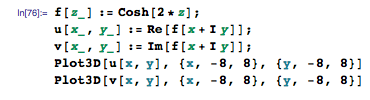
\includegraphics[scale=0.6]{task/2_15/screen1.png}
\\
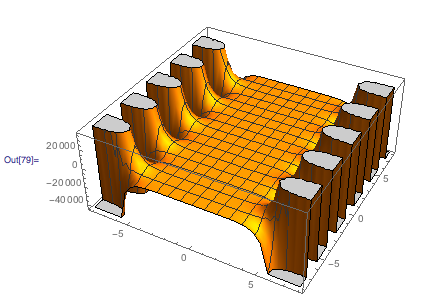
\includegraphics[scale=0.6]{task/2_15/screen2.png}
\\
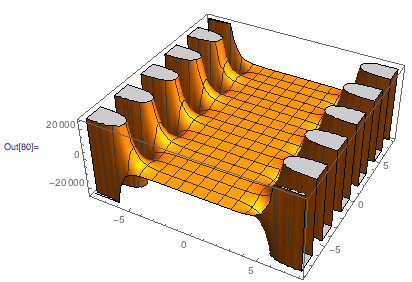
\includegraphics[scale=0.6]{task/2_15/screen3.png}
\\
Решим уравнение $ f(z) = -2 $:\\
$
	\operatorname{ch} 2z = -2
	\\[1em]
	\cos 2y \cdot \ch 2x + i \sin 2y \cdot \sh 2x = -2
	\\[1em]
	\begin{cases}
		\cos 2y \cdot \ch 2x = -2 \\
		\sin 2y \cdot \sh 2x = 0
	\end{cases}
	\\[1em]
$
Рассмотрим два случая: $ \sin 2y = 0 $ и $ \sh 2x = 0 $
\\[1em]
1 случай:
\\[1em]
$
	\ch 2x \pm 1 = -2
	\\[1em]
	\ch 2x = -2 \pm 1
	\\[1em]
	x = \pm \ch^{-1} -3; \; x = \pm \ch^{-1} -1
	\\
	y = \dfrac{\pi k}{2}, k \in \mathbb{Z}
$
\\[1em]
2 случай:
\\[1em]
$
	\sh 2x = 0
	\\[1em]
	x = 0
$
\\[1em]
Нет решений.
\subsection{Ответ:}
$
	x = \pm \ch^{-1} -3; \; x = \pm \ch^{-1} -1
	\\
	y = \dfrac{\pi k}{2}, k \in \mathbb{Z}
$
